\documentclass[11pt]{article}
\usepackage[margin=1in]{geometry}
\usepackage[T1]{fontenc}
\usepackage{lmodern}
\input{ot1lmr.fd}
\DeclareFontShape{T1}{lmr}{m}{n}{<-> ec-lmr10}{}
\DeclareFontShape{OT1}{lmr}{m}{n}{<-> rm-lmr10}{}
\input{omllmm.fd}
\DeclareFontShape{OML}{lmm}{m}{it}{<-8.5> lmmi8 <8.5-> lmmi10}{}
\input{omslmsy.fd}
\DeclareFontShape{OMS}{lmsy}{m}{n}{<-8.5> lmsy8 <8.5-> lmsy10}{}
\usepackage{amsmath,amssymb,amsthm,booktabs,graphicx,microtype}
\usepackage[hidelinks]{hyperref}
\setlength{\emergencystretch}{2em}
\clubpenalty=10000\widowpenalty=10000\displaywidowpenalty=10000
\renewcommand{\labelitemi}{$\bullet$}
\newtheorem{proposition}{Proposition}
\title{Shaping Gap Benchmark IV:\\Experience-Acquired Execution and\\Compatibility Reuse}
\author{Nathaniel Oh \and Paul Attie}
\date{November 13, 2026}
\begin{document}
\maketitle
\begin{abstract}
Can experience determine which changes to frozen neural execution are worth retaining, together with an interface that keeps existing programs usable? We close this acquisition and reuse loop over ordinary frozen pretrained transformer bodies. Native response geometry supplies candidate recurrent return updates; paired neural trajectories supply shared observation interfaces; execution feedback selects a pair to retain. In twelve runtime contexts over two model sizes, five pairs are selected and locked before two untouched validation streams. Two contexts improve nonlinear temporal processing quality by approximately 4--5\% on both streams while retaining all 13 and 18 eligible old programs, respectively. Across all twelve contexts, mean score changes are positive in both streams and 140/141 old program instances remain usable. Four selected updates improve quality on both streams with full retention; one regresses. A separate historical-feedback predictor tested on unseen runtimes misses its aggregate transfer criterion. We distinguish this result from successful experiential reuse within known contexts. Pretrained parameters, readout programs and acquired observation interfaces remain unchanged during final validation. Complete controls, unsuccessful trials and acquisition costs are released; 5,040 saved native outputs independently reproduce bit exactly. The checkpoint establishes a finite learning--execution--compatibility--reuse cycle and supplies the starting state for testing a second acquisition from an already improved runtime.
\end{abstract}

\section{Improvement as an executable pair}
A useful execution change has two obligations: make new computation accessible and keep existing computation usable. An update can satisfy the first while changing the observations expected by earlier programs. Treating the update and its compatibility interface as one acquired object makes both obligations explicit.

This paper studies that object over a complete frozen transformer body. Continuous numerical state enters the original neural computation directly. An acquired return matrix connects its response to the next invocation; a shared observation interface connects the changed response to old readout programs. The system learns which constructed pair to retain from its own execution experience and tests that choice on later input streams.

The central result is a complete finite cycle: acquire candidate execution changes, acquire their interfaces, observe outcomes, select a pair, freeze it, and reuse it on untouched inputs. Two selected pairs produce repeated quality improvement with complete old-program retention. The full cohort also contains a regression, which is retained in the evidence and the aggregate result.

Checkpoint III established preserved return augmentation and shared observation transport~\cite{sg3}. It used a fixed primary update over inherited charts. Checkpoint IV constructs twelve new charts and response geometries, tests an acquired cross-chart predictor, then closes the experiential selection loop within those contexts. Earlier checkpoints remain preserved at their original paths~\cite{sg1,sg2}.

\begin{figure}[ht]\centering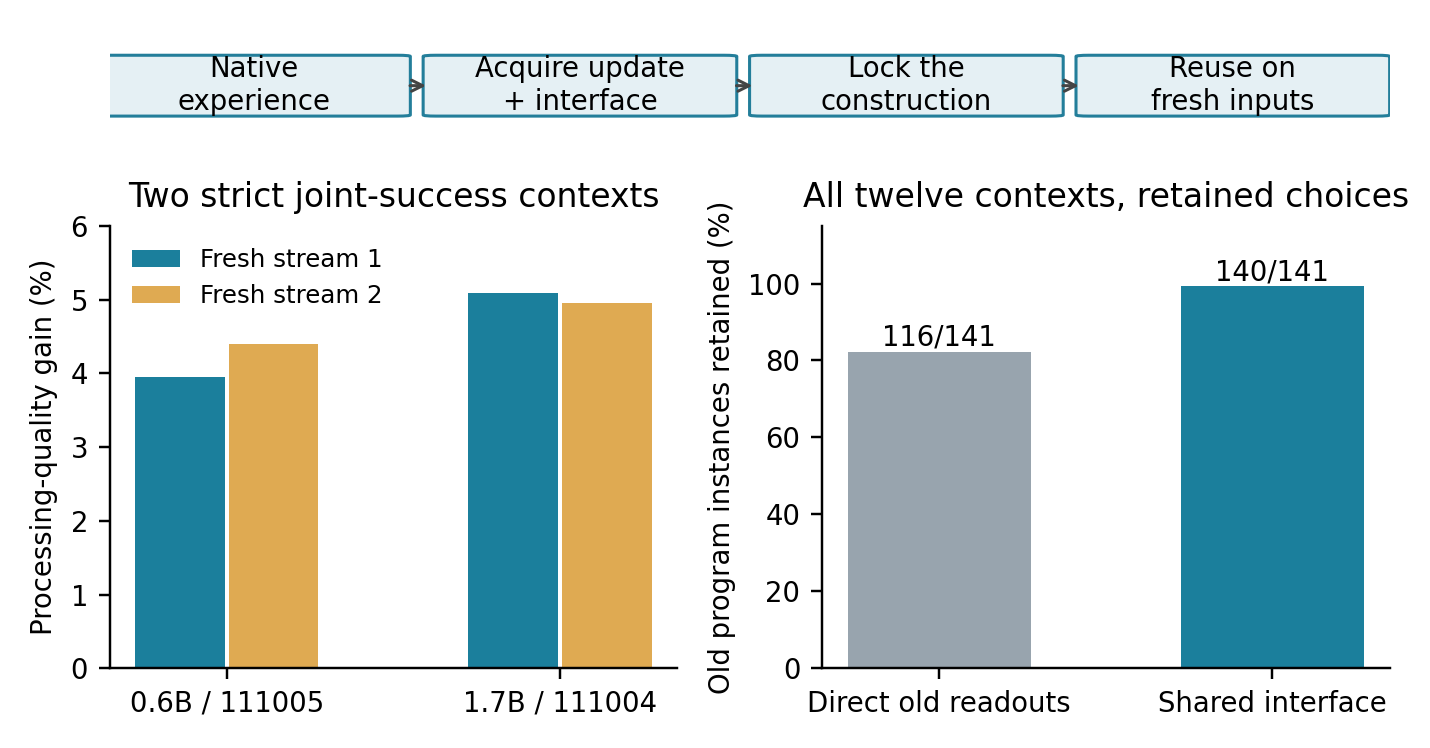
\includegraphics[width=\linewidth]{checkpoint-overview.png}
\caption{The acquired unit is an execution change together with a reusable observation interface. Left: two strict joint-success contexts. Right: old-program retention for the selected constructions across the full twelve-context cohort; baseline fallbacks are included.}\label{fig:overview}
\end{figure}

\section{Runtime and acquisition mechanism}
\subsection{The existing pretrained body is the substrate}
Let $F_\theta:\mathbb R^n\rightarrow\mathbb R^n$ denote all 28 transformer blocks and final normalization on two continuous positions. We use the pinned four-bit Qwen3-0.6B and Qwen3-1.7B MLX checkpoints, with hidden widths $h=1024$ and $h=2048$, respectively, and $n=2h$. All loaded parameter arrays remain fixed. Tokenization, English prompts and the language-generation head are outside this execution path.

A runtime chart contains a reference frame $a$, input/state directions $U_u,U_z$, scale $\epsilon$, reference response $b=F_\theta(a)$, return matrix $C\in\mathbb R^{8\times n}$ and observation projection $R\in\mathbb R^{32\times n}$. At step $t$,
\begin{align}
 x_t&=a+\epsilon(U_z^\top z_t+0.2u_tU_u^\top),\\
 y_t&=F_\theta(x_t)-b,\qquad z_{t+1}=Cy_t,\\
 \phi_t&=[z_{t+1};Ry_t]\in\mathbb R^{40}.
\end{align}
The scalar stimulus is uniform on $[-1,1]$. The frame uses two existing embedding rows as numerical starting coordinates; no linguistic interpretation of those rows is required by the method. An old program is a standardized linear readout of $\phi_t$.

\subsection{Acquire geometry and preserve the working return}
Each fresh chart is acquired using the recorded source-construction apparatus from Checkpoint III. Central differences in nine actuator directions identify a local response map $\widehat J$. Quadratic residual responses identify an output mode $q$ outside its measured first-order span and a state direction $v$. The nonlinear response projections also supply the observation basis. The source routine selects an admissible unaligned return using state participation and replica convergence. The entire native acquisition, including unselected source constructions, is charged.

The execution update preserves the working return:
\begin{equation}
 C_j=C+\alpha_jvq^\top,\qquad q^\top\widehat J\approx0.
\end{equation}
Native symmetric response probes orient the directions. A 512-step baseline source trajectory, with 128-step burn-in, calibrates the addition's return-action RMS to four signed fractions: $-5\%,-2\%,+2\%,+5\%$. Thus each candidate is a source-acquired numerical construction within a supplied family, rather than a task answer embedded in a fixed operator menu. The signed fractions, construction grammar and acquisition criterion are human-supplied.

Since $(C_j-C)\widehat J=\alpha_jv(q^\top\widehat J)$, the identified first-order map is preserved to the measured orthogonality tolerance. Higher-order and recurrent effects remain empirical questions. The fused matrix retains its original $8\times n$ shape and needs one native body invocation per step.

\subsection{Acquire a shared observation interface}
For a baseline/candidate pair driven by the same source stream, let $Y$ and $X_j$ be their standardized observation matrices. Using $N=2048$ pairs, acquire
\begin{equation}
 T_j=(X_j^\top X_j+\lambda I)^{-1}(X_j^\top Y+\lambda I),
 \qquad \lambda=0.001N.
\end{equation}
This solves least squares with an identity prior. Each side has its own source means and scales. Interface fitting uses paired neural observations, without the functional target values used for assessment.

An old readout matrix $B$ and target mean $\mu$ remain unchanged. Compatible reuse predicts $\widehat\phi_j T_jB+\mu$. Direct reuse applies the old normalization and $B$ to the changed observations without transport. One shared map serves all 143 baseline readouts for that runtime change. It is not a separate refit of each old task.

The compatibility obligation has a simple reusable form: for any old readout $w$, $|(xT-y)w|\leq\|xT-y\|_2\|w\|_2$. Checkpoint III gives the associated contract~\cite{sg3}. Source alignment does not itself establish fresh retention; the locked map and unchanged programs must execute successfully on new experience.

\section{Two learning claims, two prospective studies}
The two studies answer different questions. P61 asks whether a predictor trained on prior contexts can choose useful updates for new runtime geometry from source measurements. P62 asks whether a runtime's own execution feedback can identify a construction worth retaining for later inputs. P61's evaluation becomes explicit acquisition feedback for P62. Only the new P62 streams validate the latter reuse claim.

\subsection{P61: learned selection on unseen runtimes}
Historical training uses the four acquired signed updates in each of twelve P59 chart/model contexts: 48 rows. Each row has twenty source-derived features, including state and observation participation, variance and increment changes, trajectory cosine, held-out transport error and drift, map condition, autocorrelation, higher moments and history-reconstruction measurements. Reconstruction uses linear lag values and a fixed random Fourier encoding of sixteen-lag stimulus history. These are self-supervised source measurements; they are distinct from the 143 Legendre assessment targets.

Two prediction targets use historical functional feedback: the smaller relative quality gain across two held-out blocks, clipped to $[-2,2]$, and whether all eligible old programs are retained in both. An RBF ridge model predicts these outcomes. Six grouped folds hold out each seed identity across both model sizes. Bandwidth factors $\{0.5,1,2\}$ and ridge values $\{0.001,0.01,0.1,1\}$ are selected by grouped prediction loss. The chosen bandwidth factor is 2 and ridge is 0.01. The retained model contains 1,101 numerical values, or 8,808 bytes.

This predictor is sealed before acquiring six new charts per model size, using seeds 111001--111006. The twelve chart/model contexts have six paired seed identities; they are not twelve independently sampled model families. For each new context, a 2,304-step source stream supplies 256 washout steps and 2,048 observation pairs. The policy chooses the largest predicted gain above 1\% among candidates whose predicted complete-retention score is at least 0.5, or keeps baseline. Numerical/source-admissibility gates can force baseline. The retention score is an uncalibrated prediction score, not a certified probability.

Choices and interfaces are sealed before the new chart's functional assessment targets are generated. All assessment readouts are then trained on the source observations and frozen before two independent fresh streams. This chronology keeps new functional outcomes out of P61 selection while giving baseline and candidate readouts equal fitting opportunity.

\subsection{P62: acquire a retained pair from own experience}
P62 uses the completed P61 outcomes as development feedback in those same twelve contexts. Let $O_c$ be baseline programs reliable in both P61 blocks for context $c$. For candidate $j$, define
\begin{equation}
 g_{cj}=\min_{b\in\{1,2\}}\frac{Q_{cjb}-Q_{c0b}}{\max(Q_{c0b},0.25)}.
\end{equation}
A candidate is admissible when $g_{cj}\geq0.01$, baseline and candidate are numerically bounded in both feedback blocks, $O_c$ is nonempty, and every program in $O_c$ remains reliable through its acquired interface in both blocks. Select the admissible candidate with largest $g_{cj}$, breaking ties toward the smaller absolute action and then fixed slot order. If none is admissible, retain baseline.

This is finite empirical action selection with a supplied quality/retention contract. The acquired object is the chosen native-derived return and its shared compatibility map. Context identity is supplied; the selection rule does not claim generalization to unseen geometry. The method retains a computation, not a list of answers to future input streams.

All twelve choices are sealed before either P62 stream is generated. P62 reuses the exact P61 return matrices, normalization, observation interfaces and old/new readout coefficients. No refitting occurs during final validation. Five updates are selected and seven contexts retain baseline. Every unselected arm is also evaluated for complete controls and opportunity analysis; its later outcome cannot change the locked choice.

\section{Measurements, controls and chronology}
\subsection{Processing quality and program retention}
We use the temporal information-processing measurement construction of Dambre et al.~\cite{dambre}: 143 orthogonal Legendre-product functionals, degree one through four, of which 109 are multi-lag nonlinear targets. Standardized readouts use ridge $10^{-4}N$. The finite held-out quality score is
\begin{equation}
 Q=\sum_{j\in\mathcal M}\max(0,R_j^2),\qquad
 R_j^2=1-\mathrm{SSE}_j/\mathrm{SST}_j,
\end{equation}
where $\mathcal M$ is the 109-target nonlinear temporal subset. The reported percentages are relative changes in this score, not percentages of general model intelligence or language accuracy.

Reliability means $R^2\geq0.5$. P62 prior-old programs are reliable under the P61 baseline in both feedback blocks. The fresh reference additionally requires the unchanged baseline to stay reliable in both P62 streams. All 141 prior-old instances meet that fresh reference here, so filtered and unfiltered retention numerators/denominators coincide. Instances are counted across contexts, not as 141 distinct universal functions.

A strict fresh joint success requires at least 1\% relative quality gain in both streams, bounded baseline/candidate execution, a nonempty reference set, and retention of every reference-old program. Baseline fallback contributes zero quality gain and cannot count as acquisition. A separately recorded clarification prevents failed baselines or empty old-program sets from creating vacuous joint successes; it was recorded after the smaller P61 outcomes and larger source admissibility observations, before inspection of larger P61 functional outcomes and before any P62 validation.

\subsection{Conditions and input streams}
Each context has seven arms: baseline, four signed acquired updates, one same-source-action random $+2\%$ control, and an exact baseline clone. Every native trajectory has 42 real context/arm conditions, padded to 64 for fixed batches of 32. A state exceeding magnitude 10 or becoming nonfinite is recorded as inadmissible; subsequent state buffers are zeroed and that arm's assessment scores are set to $-1$, yielding zero positive-clipped quality. Failure times and all arms remain in the data.

P61 source seed is 112001, with a separate 512-step action calibration at seed 112101. Assessment seeds 113001 and 114001 each supply 256 washout and 2,048 scored steps from reset state. P62 repeats the same input protocol with untouched seeds 121001 and 122001. These are repeated input streams for fixed programs, not independently trained replicas.

Protocols, source versions, local registration timestamps and acquisition seals are released. They are local prospective records, not an external preregistration or independently anchored priority certificate. The initial sandboxed launch could not access Metal and executed no native sequences; the unchanged sealed policy was retried with native GPU access. No scientific condition was replaced.

\section{Results}
\subsection{New-context prediction transfers one useful construction}
P61 selects three updates on twelve new contexts. One larger-model context improves quality in both fresh blocks while retaining all fifteen eligible programs. Across all contexts, retention is 138/141, but pooled quality changes are $+0.1431$ and $-0.0148$. The declared positive-transfer criterion is therefore not met (Table~\ref{tab:transfer}). The candidate audit finds five contexts with an available strict joint-success update; the predictor captures one. This identifies useful constructions and specific selection misses without relabeling retrospective opportunities as learned choices.

\begin{table}[ht]\centering\small\begin{tabular}{lrrrrr}\toprule
Size & Updates & $\Delta_1$ & $\Delta_2$ & Joint & Old retained\\\midrule
0.6B & 2 & +0.138 & -0.067 & 0 & 68/71\\
1.7B & 1 & +0.149 & +0.038 & 1 & 70/70\\
pooled & 3 & +0.143 & -0.015 & 1 & 138/141\\
\bottomrule\end{tabular}

\caption{P61 frozen predictor on new runtime geometry. Changes include baseline fallbacks.}\label{tab:transfer}
\end{table}

\subsection{Own-experience acquisition produces fresh reuse gains}
P62 locks five updates using P61 feedback. On the two new streams, four selected updates have positive quality change in both and retain every eligible old program. Two satisfy the stricter 1\% threshold in both. The remaining smaller-model update has changes of $+4.17\%$ and $-82.91\%$ and retains two of three old programs. This adverse case remains in every pooled result.

For the 0.6B context 111005, the retained $+2\%$ update changes scores from $(11.1251,10.3585)$ to $(11.5649,10.8134)$, gains of 3.95\% and 4.39\%. Shared compatibility retains 13/13 old programs, versus 9/13 under direct reuse.

For the 1.7B context 111004, the retained $+5\%$ update changes scores from $(15.8273,16.0160)$ to $(16.6332,16.8103)$, gains of 5.09\% and 4.96\%. Shared compatibility retains 18/18 old programs, versus 10/18 under direct reuse. In both cases the source-fitted interface and readout coefficients remain fixed across feedback and final validation.

Across the entire twelve-context cohort, mean changes are $+0.11399$ and $+0.07595$ score units. Retention is 140/141, with complete retention in ten of eleven nonempty reference contexts. The twelfth context has no eligible old programs and does not count as a joint success. Direct reuse of the same selected changes retains 116/141; the shared interfaces recover 24 additional instances. These counts include unchanged-baseline fallbacks.

\begin{table}[ht]\centering\footnotesize\begin{tabular}{llrrrr}\toprule
Size & Rule & $\Delta_1$ & $\Delta_2$ & Joint & Old retained\\\midrule
0.6B & Feedback acquired & +0.082 & -0.029 & 1 & 70/71\\
0.6B & Frozen predictor & +0.097 & +0.101 & 0 & 67/71\\
0.6B & Fixed acquired +2\% & +0.259 & +0.129 & 1 & 70/71\\
0.6B & Random +2\% & +0.088 & +0.040 & 3 & 69/71\\
1.7B & Feedback acquired & +0.146 & +0.181 & 1 & 70/70\\
1.7B & Frozen predictor & +0.008 & +0.036 & 0 & 70/70\\
1.7B & Fixed acquired +2\% & -1.915 & -1.833 & 1 & 54/70\\
1.7B & Random +2\% & -0.960 & -0.863 & 0 & 59/70\\
pooled & Feedback acquired & +0.114 & +0.076 & 2 & 140/141\\
pooled & Frozen predictor & +0.052 & +0.069 & 0 & 137/141\\
pooled & Fixed acquired +2\% & -0.828 & -0.852 & 2 & 124/141\\
pooled & Random +2\% & -0.436 & -0.412 & 3 & 128/141\\
\bottomrule\end{tabular}

\caption{P62 fresh reuse: all contexts and all comparison rules. Joint means the declared strict two-stream quality/retention criterion. Frozen predictor is the unchanged P61 choice evaluated on these P62 streams.}\label{tab:aggregate}
\end{table}

The pooled feedback-acquisition criterion is met. Per-size results are heterogeneous: the smaller-model mean is positive in the first stream and negative in the second; the larger mean is positive in both. The two-stream pooled result is a finite observed outcome, rather than a population guarantee of beneficial updates.

\begin{figure}[ht]\centering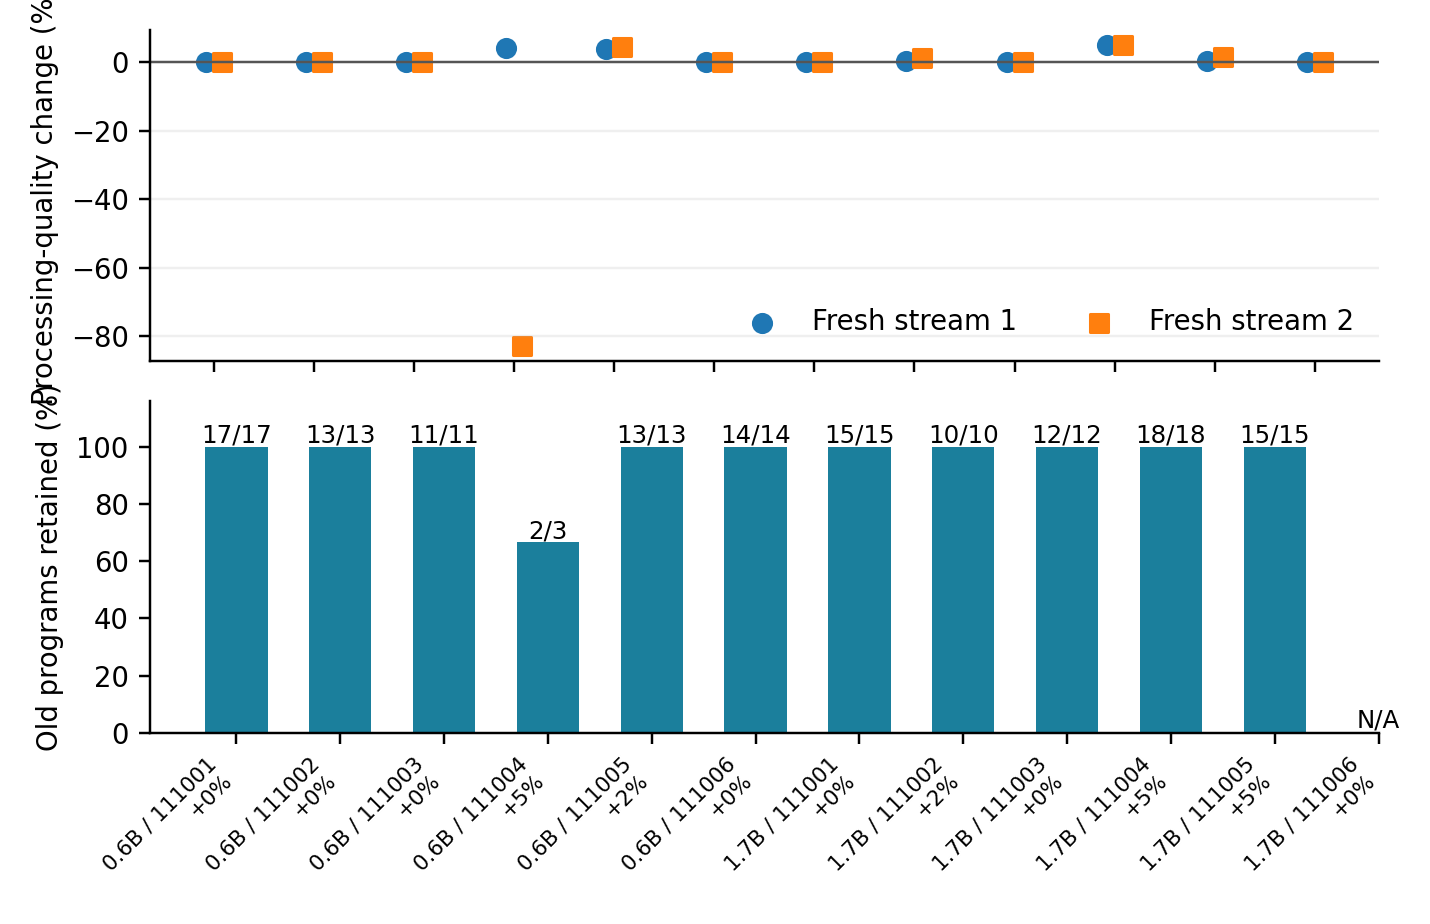
\includegraphics[width=\linewidth]{all-contexts.png}
\caption{All twelve P62 contexts, including seven baseline fallbacks, the adverse smaller update and the empty reference context. Percentages use each block's paired baseline with the declared denominator floor.}\label{fig:all}
\end{figure}

\subsection{Controls and the meaning of the advance}
The fixed acquired $+2\%$ rule has pooled changes $-0.8281,-0.8524$ and retains 124/141 old instances on P62 streams. The primary random $+2\%$ rule has changes $-0.4357,-0.4117$ and retains 128/141. That random control has three strict joint-success contexts, versus two for feedback selection, while its aggregate quality and retention are worse. Thus counts of isolated successes and whole-cohort performance answer different questions. Selected $+5\%$ constructions do not have a same-dose random control in this study, so these comparisons do not establish directional superiority at that selected dose.

No selected update satisfies the stronger newly reliable nonlinear-target criterion across all four feedback/validation blocks: treatment reliable in all four, baseline below threshold in all four. The random control has one such target instance. The demonstrated advance is repeatable processing-quality improvement with retained computational access, with reliable new-functional-class acquisition tracked separately.

\section{Acquisition, retained state and lifecycle cost}
The full prior checkpoint ledger contains 834,732 inherited P55/P56 source sequences plus 1,413,312 P59/P60 and verification sequences. P59 provides the historical predictor's training labels; P60 is earlier instrument development, not additional predictor training data. P61 adds 1,254,764 sequences; P62 adds 589,824; independent current verification adds 7,680. Current new work totals 1,852,268 two-position sequences. Including the complete recorded prior ledger gives 4,100,312 sequences. Publication validation of the portable entrypoint repeats the saved-output checks for another 7,680 native sequences, separately recorded as release QA; it does not add independent scientific observations. Pretraining is inherited and electrical energy was not measured.

\begin{table}[ht]\centering\small\begin{tabular}{llrrr}\toprule
Study & Size & Native sequences & Wall s & Peak RSS MiB\\\midrule
P61 & 0.6B & 627,382 & 329.6 & 687.5\\
P61 & 1.7B & 627,382 & 795.6 & 1433.9\\
P62 & 0.6B & 294,912 & 153.1 & 645.5\\
P62 & 1.7B & 294,912 & 376.9 & 1386.9\\
\bottomrule\end{tabular}

\caption{Recorded experiment work, wall time and whole-process peak RSS. Native verification is separately charged; full source/fit/assessment subdivisions are in the ledger.}\label{tab:cost}
\end{table}

All native chart acquisition, source exploration, unused updates, clones, padding and outcome feedback are charged. The predictor fit takes approximately 0.99 seconds in the recorded environment. Interface/diagnostic fitting takes approximately 0.21 seconds per size after source trajectories are available. These small fitting times do not erase the native experience cost. Exploring four candidates requires more logical source work than trying one fixed update; shared experimental exposure is not equal minimal acquisition cost.

The fused return contains 16,384 or 32,768 float64 coefficients, occupying 131,072 or 262,144 bytes. The shared interface adds 1,600 coefficients (12,800 bytes) and 160 serialized normalization values (1,280 bytes). The predictor retains 8,808 bytes. Each full 143-program readout library occupies 47,544 bytes, including coefficients and normalization; old and candidate libraries are explicitly counted as assessment programs. Reusing old programs retains their arrays. Deploying new decoded outputs also retains the corresponding new readout vectors.

Recorded full chart arrays occupy 1,015,872 and 2,031,680 bytes, including acquisition geometry and access constants. These are conservative stored-chart measurements, not a minimal deployed representation. The model arrays occupy approximately 317 and 914 million bytes, and whole-process peaks are reported separately. Fixed return shape and eight-state recurrence describe the deployed computational core; they do not claim fixed total storage for an arbitrarily growing archive. A selected interface adds affine observation work while native body calls per recurrent step remain one.

\section{Building blocks and the measured contribution}
Temporal capacity measurements provide established instruments for evaluating dynamical computation~\cite{dambre}. Frozen pretrained transformers have been adapted to non-language tasks while retaining core components~\cite{lu}. Model stitching learns trainable connections between fixed representations~\cite{stitch}. These supply direct foundations for the substrate, measurement and compatibility components used here.

Our ridge alignment, RBF prediction, finite empirical action selection and observer inequalities are standard machinery. The contribution is the executable acquired unit and the closed experimental loop: source-derived neural execution changes paired with shared compatibility, experiential selection, frozen reuse on new streams, unchanged-program assessment and a complete cost ledger. It extends the preserved-update mechanism of Checkpoint III~\cite{sg3} with fresh native geometry acquisition and selection/reuse evidence. The negative new-context transfer result stays separate from the positive within-context reuse result.

\section{From one acquired improvement to cumulative development}
This checkpoint supplies two retained execution/interface pairs with repeated quality gains and complete old-program reuse on untouched streams. It also supplies the failed selection, unstable conditions and one fresh regression needed to develop stronger applicability contracts.

The next experiment can begin from an already accepted updated runtime, acquire another change, and ask whether it adds a second retained gain. Affine compatibility maps can be composed into one fixed-size map, with error propagation, fitting, rejected trials and maintenance charged. That is the direct test of cumulative development suggested by the present result. Reliable new-context selection and newly reliable functional classes remain measurable acquisition targets rather than consequences assumed from one positive cycle.

\appendix
\section{All retained choices and fresh outcomes}
\begin{table}[ht]\centering\small\begin{tabular}{llrrrrl}\toprule
Size & Seed & Action & $\Delta_1$ & $\Delta_2$ & Retained & Joint\\\midrule
0.6B & 111001 & +0\% & +0.000 & +0.000 & 17/17 & --\\
0.6B & 111002 & +0\% & +0.000 & +0.000 & 13/13 & --\\
0.6B & 111003 & +0\% & +0.000 & +0.000 & 11/11 & --\\
0.6B & 111004 & +5\% & +0.052 & -0.628 & 2/3 & --\\
0.6B & 111005 & +2\% & +0.440 & +0.455 & 13/13 & yes\\
0.6B & 111006 & +0\% & +0.000 & +0.000 & 14/14 & --\\
1.7B & 111001 & +0\% & +0.000 & +0.000 & 15/15 & --\\
1.7B & 111002 & +2\% & +0.025 & +0.077 & 10/10 & --\\
1.7B & 111003 & +0\% & +0.000 & +0.000 & 12/12 & --\\
1.7B & 111004 & +5\% & +0.806 & +0.794 & 18/18 & yes\\
1.7B & 111005 & +5\% & +0.045 & +0.213 & 15/15 & --\\
1.7B & 111006 & +0\% & +0.000 & +0.000 & 0/0 & --\\
\bottomrule\end{tabular}

\caption{All twelve P62 retained choices. Action is source return-action fraction; $\Delta$ is fresh nonlinear temporal score change. The zero-reference row is retained and cannot be a joint success.}\label{tab:cases}
\end{table}
Complete score vectors for every candidate, block and comparison are released, together with the P61 historical predictor features, targets, hyperparameter grid, frozen parameters and P62 selection feedback. A retrospective P62 opportunity analysis finds four contexts with an available strict joint-success construction; the locked feedback policy captures two. Those opportunities are not substituted for the policy's actual outcomes.

\section{Reproduction and integrity}
Independent replay reconstructs functional targets with a separate Legendre implementation, applies frozen readouts, refits the shared transports and predictor, recomputes all choices, and checks 387 acquisition/retention seals. It reproduces 1,008 score vectors; maximum absolute $R^2$ differences are $6.99\times10^{-10}$ and $4.66\times10^{-10}$ for P61 and P62. Transport and predictor refits agree exactly in the recorded analysis environment.

\begin{samepage}
Original-weight re-execution independently reproduces 5,040 saved native output vectors bit exactly: 3,024 for P61 and 2,016 for P62. Loaded-parameter digests agree before and after. The native environment uses NumPy 2.5.4, MLX 0.32.4 and MLX-LM 0.32.2 on an Apple M4 Max with 36 GiB memory. Other platforms should record numerical tolerances rather than assume identical bits.
\end{samepage}

The pinned model revisions are:
\begin{quote}\small
0.6B: \texttt{173234aa840d113125e9f2271100ddbaf16c9620}\\
1.7B: \texttt{21457c6f51ed54a7c16e988c0844db973815c137}
\end{quote} The repository guide provides model-free replay, optional original-weight verification and a separate native acquisition workspace that reuses the preserved historical checkpoint data. Weights are downloaded separately. Publication changes only machine-local checkpoint receipt paths to portable model paths; transformations and hashes are recorded, and numeric NPZ payloads remain unchanged.

\begin{thebibliography}{6}\raggedright
\bibitem{sg1} N. Oh and P. Attie. Shaping Gap Benchmark: Effect Interfaces for Compositional Execution of Frozen Neural Computation. Repository paper, 2026. \url{https://github.com/calysteon/shaping-gap-benchmark/blob/main/paper/shaping-gap-benchmark.pdf}.
\bibitem{sg2} N. Oh and P. Attie. Shaping Gap Benchmark II: Scalable Effect-Interface Evaluation and Verified Functional Construction. Repository paper, 2026. \url{https://github.com/calysteon/shaping-gap-benchmark/tree/main/checkpoints/02-scaling-and-functions}.
\bibitem{sg3} N. Oh and P. Attie. Shaping Gap Benchmark III: Preserved Neural Augmentation and Reusable Observation Interfaces. Repository paper, 2026. \url{https://github.com/calysteon/shaping-gap-benchmark/tree/main/checkpoints/03-preserved-neural-augmentation}.
\bibitem{dambre} J. Dambre, D. Verstraeten, B. Schrauwen and S. Massar. Information Processing Capacity of Dynamical Systems. \emph{Scientific Reports} 2, 514, 2012. \url{https://doi.org/10.1038/srep00514}.
\bibitem{lu} K. Lu, A. Grover, P. Abbeel and I. Mordatch. Pretrained Transformers as Universal Computation Engines. 2021. \url{https://arxiv.org/abs/2103.05247}.
\bibitem{stitch} Y. Bansal, P. Nakkiran and B. Barak. Revisiting Model Stitching to Compare Neural Representations. \emph{NeurIPS}, 2021. \url{https://arxiv.org/abs/2106.07682}.
\end{thebibliography}
\end{document}
